\chapter{Лабораторная работа №7. Реализация корреляционного устройства на ПЛИС}

\section{Сжатие сигналов с применением быстрой свёрки}

Сжатие сигналов — это метод обработки сигналов, используемый в радиолокационных системах,
позволяет максимизировать отношение сигнал/шум и получить высокое разрешение воспринимаемого объекта (например, для достижения чувствительного обнаружения цели или хорошего качества изображения). Принцип действия радиолокационной аппаратуры заключается в облучении объекта радиоволнами и приёме отражённого от него сигнала (см. рисунок). Для обнаружения и определения местоположения самолёта, корабля, крупного населённого пункта или иного объекта радиолокационная станция должна выработать электромагнитную энергию, излучить её в нужном направлении, принять и зарегистрировать отражённый от объекта сигнал. Местоположение объекта, отражающего радиоволны, определяют путём измерения дальности до этого объекта и направлении на него.

Наиболее широко применяемый в настоящее время метод измерения дальности - импульсный. При таком методе радиолокационная станция излучает электромагнитную энергию не непрерывно, а короткими импульсами, измеряемыми единицами и даже долями микросекунды. После посылки импульса радиоволн станция некоторое время работает только на приём, улавливая и регистрируя отражённый сигнал. Затем станция излучает следующий импульс и вновь переключается на приём.

По времени прохождения сигнала от станции до объекта и обратно определяют расстояние до объекта: чем больше дальность, тем больше требуется времени, чтобы импульс достиг объекта, отразился от него и возвратился обратно.

Измерив промежуток времени t между моментом излучения станцией импульса и моментом приёма отражённого сигнала, и зная скорость распространения радиоволн (с достаточной степенью точности её можно принять равной 300000 км/сек), нетрудно подсчитать расстояние $R$ до отражающего объекта по формуле:
\begin{equation}
R = \frac{c \cdot \tau}{2},
\end{equation}
Цифра 2 в знаменателе формулы характеризует двойной путь сигнала - от радиолокационной станции до объекта и обратно.

Современных решением для сжатия сложных сигналов является цифровая быстрая свёртка в спектральной области на основе БПФ. Алгоритм быстрой свёртки имеет следующий вид:

\begin{equation}	
	y(k) = IFFT[FFT\{x(k)\} \cdot \compconj{FFT\{S(k)\}}],
\end{equation}

где y(k) - отсчёты сжатаго сигнала; x(n) - отсчёты эхо-сигналов, то есть отражённый от целей; S(k) - отсчёты, описывающие зондирующий сигнал(опорная функция). Блок-схема алгоритма приведена на рисунке ~\ref{fft_conv}.

\begin{figure}[h]
	\centering
	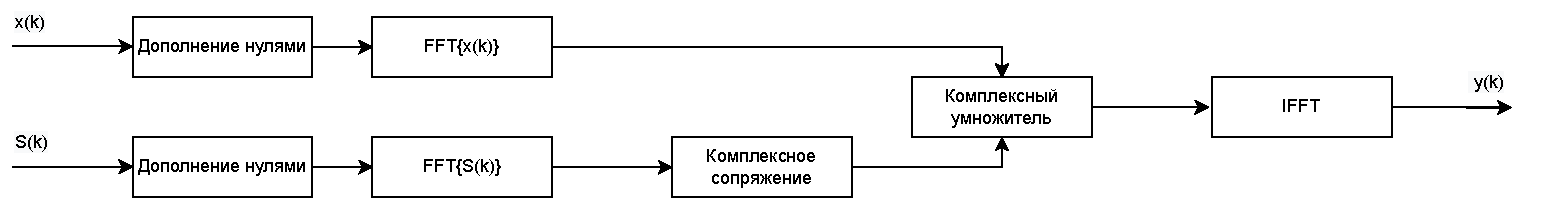
\includegraphics[width=0.9\textwidth]{fft_conv.pdf}
	\caption{Блок-схема алгоритма быстрой свёртки}
	\label{fft_conv}
\end{figure}

Данный алгоритм сжатия (свертки) сложных сигналов и сама система сжатия имеет большие преимущества перед согласованными фильтрами, так как легко адаптируется к виду сигнала, его ширине спектра, обладает большим динамическим диапазоном и легко реализуется при использовании современных цифровых компонентов, особенно программируемых логических интегральных схем (ПЛИС).

В РЛС широкое применение получили сигналы с линейной-частотной модуляцией(ЛЧМ), а также импульсные сигналы с фазокодовой бинарной модуляцией(ФКМ). Рассмотрим процесс сжатия на примере данных сигналов.

Сигнал с линейной-частотной модуляцией определяется по следующей формуле:
\begin{equation}	
	s(t) = rect(\frac{t}{T}) \cdot \cos(2 \cdot \pi \cdot f_0 \cdot t + j \cdot \pi \cdot K \cdot t^{2}),
\end{equation}

где t - время в секундах, K-скорость изменения частоты во времени, T - длительность импульса, rect() - прямоугольное окно, \(f_0\) - несущая частота.

После прохождения через квадратурный демодулятор получаем следующий комплексный сигнал:

\begin{equation}	
	g(t) = rect(\frac{t}{T}) \cdot \exp(j \cdot \pi \cdot K \cdot t^{2})
\end{equation}

Действительная часть называется квадратурной
составляющей ЛЧМ-сигнал, и обозначается как \(Q(t)\), а мнимая 
синфазной составляющей ЛЧМ-сигнала, и обозначается как \(I(t)\):

\begin{equation}	
	Q(t) = rect(\frac{t}{T}) \cdot \cos(\pi \cdot K \cdot t^{2}),
\end{equation}

\begin{equation}	
	I(t) = rect(\frac{t}{T}) \cdot \sin(\pi \cdot K \cdot t^{2}).
\end{equation}

Важнейшими параметрами ЛЧМ-сигнала являются:

\begin{enumerate}
	\item Девиация частоты: 
\begin{equation}
	BW = |K| \cdot T, 
\end{equation}
измеряется в Гц.
	\item База: 
\begin{equation}
	B = |K| \cdot T^2, 
\end{equation}
безразмерная величина.
\end{enumerate}

\begin{figure}[h]
    \centering
    \noindent
    \begin{tikzpicture}
        \begin{axis}
            [
            RCS Plot,
            title={},
            height=0.35\textwidth,
            xlabel={Время, мкс},
            ylabel={Амплитуда, отсчётов},
            legend pos = south east
            ]
            \addplot table {Synopsis/data/third-party/lfm_im.dat};
            \addlegendentry{Q(t)};
            \addplot table {Synopsis/data/third-party/lfm_re.dat};
            \addlegendentry{I(t)};
        \end{axis}
    \end{tikzpicture}
    \caption{Квадратурная и синфазная составляющая ЛЧМ сигнала}
    \label{fig:chirp}
\end{figure}

Рассмотрим конкретный пример демодулированного ЛЧМ-сигнала. Пусть он имеет следующие параметры: девиация частоты \(BW\) = 400 МГц, длительность сигнала \(T\) = 4 мкс. При этом считаем, что частота дискретизации аналого-цифрового преобразователя(АЦП) в каждом квадратурном канале(то есть мы дискретизируем по времени и квадратурную и синфазную) составляет \(F_{D}\) = 1000 МГц. На рисунке ~\ref{fig:chirp} представлена квадратурная и синфазная составляющая ЛЧМ-сигнала с приведёнными выше параметрами.

\begin{figure}[h]
    \centering
    \noindent
    \begin{tikzpicture}
        \begin{axis}
            [
            RCS Plot,
            title={},
            height=0.35\textwidth,
            xlabel={Время, мкс},
            ylabel={Амплитуда, отсчётов},
            legend pos = south east
            ]
            \addplot table {Synopsis/data/third-party/lfm_shift_im.dat};
            \addlegendentry{Q(t)};
            \addplot table {Synopsis/data/third-party/lfm_shift_re.dat};
            \addlegendentry{I(t)};
        \end{axis}
    \end{tikzpicture}
    \caption{Квадратурная и синфазная составляющая задерженного ЛЧМ сигнала}
    \label{fig:chirp_shift}
\end{figure}

Проведём моделирование отражённого от цели сигнала. При распространении сигнала возникает временная задержка, накладывается шум, а также происходит затухание сигнала. Введём некоторую временную задержку, а также наложим на сигнал белый шум. При наложении белого шума будем руководствоватся заданным отношение сигнал/шум на уровне 0 Дб. На рисунке~\ref{fig:chirp_shift} представлена сдвинутая по времени копия ЛЧМ-сигнала, а на рисунке~\ref{fig:chirp_shift_noise} представлен этот же сдвинутый сигнал, но уже при наличии шума.  

Проведём сжатие данного сигнала на основе формулы представленной в предыдущем параграфе. Для этого:

\begin{enumerate}
	\item Находим быстрое преобразование Фурье эталонного сигнала(рис. ~\ref{fig:chirp}), выполняем комплексное сопряжение полученного массива.
	\item Находим быстрое преобразование Фурье отражённого от цели (в терминах радиолокации) сигнала (рис. ~\ref{fig:chirp_shift_noise}).
	\item Производим комплексное умножение полученных массивов.
	\item Находим обратное быстрое преобразование Фурье.
\end{enumerate}

\begin{figure}[h]
    \centering
    \noindent
    \begin{tikzpicture}
        \begin{axis}
            [
            RCS Plot,
            title={},
            height=0.35\textwidth,
            xlabel={Время, мкс},
            ylabel={Амплитуда, отсчётов},
            legend pos = south east
            ]
            \addplot table {Synopsis/data/third-party/lfm_shift_noise_im.dat};
            \addlegendentry{Q(t)};
            \addplot table {Synopsis/data/third-party/lfm_shift_noise_re.dat};
            \addlegendentry{I(t)};
        \end{axis}
    \end{tikzpicture}
    \caption{Квадратурная и синфазная составляющая задержненного ЛЧМ сигнала при наличии шума}
    \label{fig:chirp_shift_noise}
\end{figure}

\begin{figure}[h]
    \centering
    \noindent
    \begin{tikzpicture}
        \begin{axis}
            [
            RCS Plot,
            title={},
            height=0.35\textwidth,
            xlabel={Время, мкс},
            ylabel={Амплитуда, отсчётов},
            legend pos = south east
            ]
            \addplot table {Synopsis/data/third-party/correl_re.dat};
            \addlegendentry{I(t)};
			\addplot table {Synopsis/data/third-party/correl_im.dat};
            \addlegendentry{Q(t)};
        \end{axis}
    \end{tikzpicture}
    \caption{Квадратурная и синфазная составляющая сигнала на выходе фильтра сжатия}
    \label{fig:correl}
\end{figure}

На рисунке ~\ref{fig:correl} представлены квадратурная и синфазная составляющая сжатого сигнала. При этом прослеживается чёткий пик, не смотря на наличие шума. Эта помехоустойчивость достигается за счет того, что фильтр согласуется только с сигналом, а не с шумом — он не коррелирует с шумом. Согласованный фильтр «собирает» большую часть компонентов сигнала в один пик, но оставляет шумовые компоненты случайным образом распределенными в выходном массиве. Известно, что при наличии гауссовского аддитивного шума оптимальным приемником с точки зрения максимизации отношения сигнал/шум на пике сжатого импульса является приемник с согласованным фильтром.

В отличие от непрерывных сигналов с линейной частотной модуляцией, сигналы с фазокодовой модуляцией относятся к классу дискретных сигналов, которые составляются из элементарных импульсов (дискретов), фаза или частота которых изменяются от импульса к импульсу дискретно в соответствии с определенной кодовой последовательностью. Если несущая частота зондирующего импульса остается неизменной, а начальная фаза элементарных импульсов имеет два значения 0 и $\pi$, то такие дискретные сигналы называются бинарными фазоманипулированными или сигналами с фазокодовой бинарной модуляцией (ФКМ-сигналы). Основные свойства фазоманипулированных сигналов определяются кодом, который применен для модуляции. Аналитически ФКМ-сигнал с бинарной модуляцией 0/п может быть представлен в виде [7.7]:

\begin{equation}
    S(t) = A_{0}\sum_{k=1}^{N} C_{k}\cos(\omega_{0}t),   0 <= t <= T;
\end{equation}

S(t)= 0, вне интервала $T$; где $A_{0}$ - амплитуда зондирующего сигнала, N - число символов кодовой последовательности (база сигнала); $T_{и} = N \cdot \tau_{0}$ - длительность зондирующего импульса; $\tau_{0}$ - длительность символа кодовой последовательности;  $\omega_{0}$ - несущая частота зондирующего сигнала; k - номер символа (дискрета) кодовой последовательности; $C_{k}$ значение символа кодовой последовательности, равное $\pm1$.

Выражение (7.6) составлено с учетом того, что:

Символы кодовой последовательности $C_{k}$ принимают значения $\pm1$ эквивалентные фазовой манипуляции несущей $0/\pi$, если $(k - 1)\tau_{0} < t < k\tau_{0}$, и $C_{k} = 0$ в остальных случаях.

В данной лабораторной работе в качестве кодовых последовательностей рассматривается их конкретная разновидность так называемые М-последовательности (МП), свойства которых хорошо изучены и описаны в научной литературе. Эти последовательности также называют последовательностями максимальной длины (периода) или последовательностями Хаффмана.

Основными параметрами одиночных M-последовательностей являются следующие:

1) длительность элементарного символа последовательности величина, обратная тактовой частоте Fi;

\begin{enumerate}
    \item Выбирается первообразный неприводимый над полем GF(2) полином степени n:
    \begin{equation}
    f(x) = x^{n} + a_{n-1}x^{n-1} + ... + a_{x}x + a_{0}
    \end{equation}
    \item Составляем сопровождающую матрицу:
    \begin{equation} 
    H = 
        \begin{bmatrix}
            0 & 0 & .. & 0 & a_{0}\\
            1 & 0 & .. & 0 & a_{1}\\
            0 & 1 & .. & 0 & a_{2}\\
            .. & .. & .. & .. & ..\\
            0 & 0 & .. & 0 & a_{n-2}\\
            0 & 0 & .. & 1 & a_{n-1}
        \end{bmatrix}.
    \end{equation}
    \item Вычисляем векторы:
    \begin{equation}
        x^{(i + 1)} = H \cdot x^{i}, 
    \end{equation}
    \begin{equation}
        x^{0} =
        \begin{bmatrix}
            1 \\
            0 \\
            0 \\
            ..\\
            0 \\
            0 
        \end{bmatrix}, 
    \end{equation}
    \begin{equation}
        i = 0, 1, ... n - 2
    \end{equation}
    \item Из полученной матрицы X формируем код:
\end{enumerate}

\begin{figure}[h]
    \centering
    \noindent
    \begin{tikzpicture}
        \begin{axis}
            [
            RCS Plot,
            title={},
            height=0.35\textwidth,
            xlabel={Время, мкс},
            ylabel={Амплитуда, отсчётов},
            legend pos = south east
            ]
            \addplot table {Synopsis/data/third-party/m_seq_re_sf.dat};
            \addlegendentry{Q(t)};
            \addplot table {Synopsis/data/third-party/m_seq_im_sf.dat};
            \addlegendentry{I(t)};
        \end{axis}
    \end{tikzpicture}
    \caption{Квадратурная и синфазная составляющая задержненного ЛЧМ сигнала при наличии шума}
    \label{fig:chirp_shift_noise}
\end{figure}

\begin{figure}[h]
    \centering
    \noindent
    \begin{tikzpicture}
        \begin{axis}
            [
            RCS Plot,
            title={},
            height=0.35\textwidth,
            xlabel={Время, мкс},
            ylabel={Амплитуда, отсчётов},
            legend pos = south east
            ]
            \addplot table {Synopsis/data/third-party/m_seq_re_recv.dat};
            \addlegendentry{I(t)};
            \addplot table {Synopsis/data/third-party/m_seq_im_recv.dat};
            \addlegendentry{Q(t)};
        \end{axis}
    \end{tikzpicture}
    \caption{Квадратурная и синфазная составляющая сигнала на выходе фильтра сжатия}
    \label{fig:correl}
\end{figure}

\begin{figure}[h]
    \centering
    \noindent
    \begin{tikzpicture}
        \begin{axis}
            [
            RCS Plot,
            title={},
            height=0.35\textwidth,
            xlabel={Время, мкс},
            ylabel={Амплитуда, отсчётов},
            legend pos = south east
            ]
            \addplot table {Synopsis/data/third-party/correl_re_m_seq.dat};
            \addlegendentry{I(t)};
            \addplot table {Synopsis/data/third-party/correl_im_m_seq.dat};
            \addlegendentry{Q(t)};
        \end{axis}
    \end{tikzpicture}
    \caption{Квадратурная и синфазная составляющая сигнала на выходе фильтра сжатия}
    \label{fig:correl}
\end{figure}

\begin{figure}[h]
    \centering
    \noindent
    \begin{tikzpicture}
        \begin{axis}
            [
            RCS Plot,
            title={},
            height=0.35\textwidth,
            xlabel={Время, мкс},
            ylabel={Амплитуда, отсчётов},
            legend pos = south east
            ]
            \addplot table {Synopsis/data/third-party/lfm_freq.dat};
            \addlegendentry{I(t)};
        \end{axis}
    \end{tikzpicture}
    \caption{Квадратурная и синфазная составляющая сигнала на выходе фильтра сжатия}
    \label{fig:correl}
\end{figure}


\section{Выполнение быстрого преобразование Фурье на ПЛИС}

Для реализации БПФ на ПЛИС используем стандартное ядро, которое предоставляет Xilinx.

\subsection{Возможности ядра}

Ядро вычисляет N-точечное дискретное преобразование Фурье(как прямое, так и обратное), где N может быть равно $2^m$, m = 3–16. Входные данные должны быть всегда представлены в естественном порядке, а выходные данные могут быть либо в естественном, либо в обратном порядке битов/цифр. Алгоритм БПФ переупорядочивает входные данные во время обработки таким образом, что данные, вводимые в естественном порядке, выводятся в бит-реверсном порядке. Заметим что вывод в естестенном порядке требует дополнительного времени преобразования и дополнительных ресурсов на ПЛИС.  

Входные данные могут быть как в формате с фиксированной точкой, так и в формате с плавающей точкой одинарной точности(по факту это реализация с фиксированной точкой с достижение шумовых характеристик плавающей точки одинарной точности). В обоих режимах входные данные представляют собой вектор из N комплексных значений. 

Размер обрабатываемого вектора данных N, выбор прямого или обратного преобразования, параметры масштабирования и длина циклического префикса могут настраиваться во время выполнения. Тип преобразования (прямое или обратное), параметры масштабирования и длину циклического префикса можно изменять для каждого кадра. Изменение же размера обрабатываемых данных N приведёт к сбросу ядра. 

Ядро БПФ предлагает четыре варианта архитектуры, обеспечивающие компромисс между ресурсами, которые будет занимать ядро на ПЛИС и пропускной способностью ядра (как правило, каждая архитектура предлагает двухкратную разницу в ресурсах по сравнению со следующей архитектурой): 

\begin{enumerate}
	\item Конвейерный потоковый ввод-вывод(Pipelined Streaming I/O) — обеспечивает непрерывную обработку данных. 
	\item Radix-4 — загружает и обрабатывает данные отдельно, используя итеративный подход. Оно меньше по размеру, чем конвейерное решение, но имеет большее время преобразования. 
	\item Radix-2 — использует тот же итеративный подход, что и Radix-4, но бабочка меньше. Это означает, что он меньше по размеру, чем решение Radix-4, но время преобразования больше. 
	\item Radix-2 Lite Burst I/O — основанный на архитектуре Radix-2, этот вариант использует подход с временным мультиплексированием к бабочке для еще меньшего ядра за счет более длительного времени преобразования.
\end{enumerate} 

\begin{figure}[h]
	\centering
	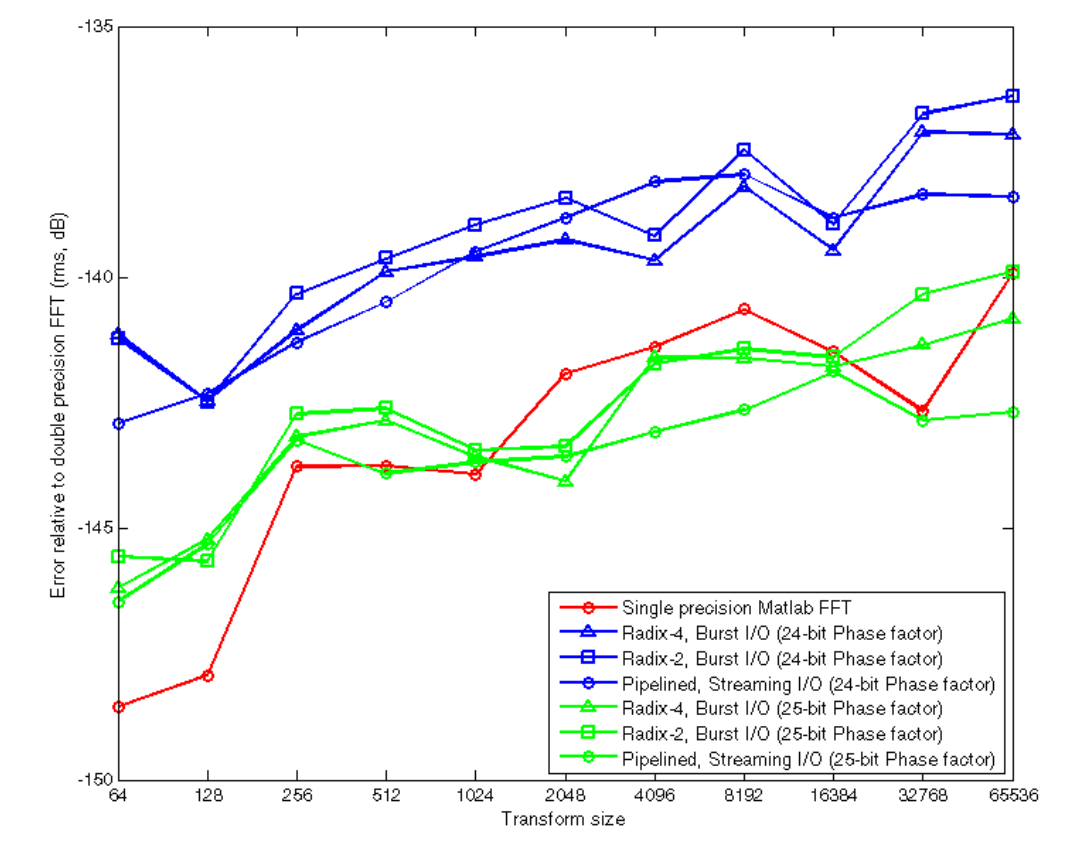
\includegraphics[width=0.6\textwidth]{image/fft_xilinx_fp.png}
	\caption{Сравнение двух уровней шумовых характеристик}
	\label{fft_xilinx_fp}
\end{figure}

Ядро БПФ может принимать данные в формате одинарной точности IEEE-754 с 32-битными словами, состоящими из 1-бита знака, 8-битной экспоненты и 23-битной дроби. Реализация полной плавающей точки на ПЛИС является дорогостоящей с точки зрения требуемых ресурсов. Режим с плавающей точкой использует БПФ с фиксированной запятой более высокой точности для достижения шумовых характеристик, аналогичных полному БПФ с плавающей точкой, со значительно меньшими ресурсами. Рисунок~\ref{fft_xilinx_fp} иллюстрирует два возможных уровня шумовых характеристик при выборе 24 или 25 битов для ширины фазового коэффициента. При увеличении ширины фазового коэффициента до 25 бит может потребоваться больше ресурсов в зависимости от целевого устройства. Таким образом для достижения наибольшей точности вычислений в режиме с плавающей точкой требуется выбирать ширину фазового коэффициента равной 25 бит при наличии ресурсов необходимых для этого.

При использовании ядра БПФ в проекте неизбежно возникает вопрос моделирования полученной схемы в симуляторе. Однако моделирование ядра требует больших затрат времени. Для ускрорения этого процесса можно использовать С-модель ядра, которая с точностью до бита воспроизводит выходные данные во всех режимах работы. Также модель БПФ доступна как MEX-функция программного обеспечения MATLAB.

\subsection{Интерфейс настройки ядра и сигналы событий}

Размер входного вектора обрабатываемых данных, длина циклического префикса(если используется), тип преобразования (прямое или обратное) и коэффициенты маштабирования данных(при использовании вычислений с фиксированной точкой) задаются с использованием интерфейс AXI4-Stream под названием \verb|S_AXIS_CONFIG|. 
Он состоит из следующих линий ввода/вывода: 

\begin{enumerate}
	\item \verb|s_axis_data_tdata| - шина данных;
	\item \verb|s_axis_config_tvalid|, \verb|s_axis_config_tready| - линии механизма "рукопожатий" в интерфейсе AXI4.
\end{enumerate}

Поля конфигурации упаковываются в вектор \verb|s_axis_config_tdata| в следующем порядке (начиная с младшего разряда):

\begin{enumerate}
	\item Поле \verb|NFFT| и дополнение нулями. Значение \verb|NFFT| равно log2 (размер преобразуемого вектора данных). Размер преобразуемого вектора данных N может быть размером максимального преобразования(выбирается при настроке в графическом интерфейсе) или любым меньшим размером. Например, 1024-точечное БПФ может вычислять размеры 1024, 512, 256 и т. д. Это поле присутсвует только при выборе режима Run time configurable transform length. Если введенное значение NFFT слишком велико, ядро устанавливает максимально доступный размер точки. Если значение слишком мало, ядро устанавливает наименьший доступный размер точки: 64 для архитектуры Burst I/O Radix-4 и 8 для других архитектур. 
	\item Длина циклического префикса \verb|CP_LEN| и дополнение нулями.
	\item Выбор типа преобразования - прямое или обратное. Когда \verb|FWD_INV| = 1, вычисляется прямое преобразование. Если \verb|FWD_INV| = 0, вычисляется обратное преобразование. Поле содержит 1 бит на канал данных БПФ, бит 0 (LSB) представляет канал 0, бит 1 представляет канал 1 и т. д.
	\item Коэффициенты маштабирования данных - \verb|SCALE_SCH|. При использовании данных с фиксированной точкой возможно маштабирование, при использовании плавающей точки одинарной точности оно игнорируется.
\end{enumerate}

Также в ядре присутствуют следующие сигналы событий:

\begin{enumerate}
	\item \verb|event_frame_started| принимает значение логической единицы на один такт, когда ядро начинает обрабатывать новый пакет. Этот сигнал предназначен для подсчета кадров и синхронизации конфигурации ядра с конкретным кадром, если это необходимо.
	\item \verb|event_tlast_missing| принимает значение логической единицы на один такт, когда \verb|s_axis_data_tlast| имеет значение логического нуля для последнего отчёта входящего пакета.
	\item \verb|event_tlast_unexpected| принимает значение логической единицы на один такт, когда ядро видит \verb|s_axis_data_tlast| в состоянии логической единицы для любого отсчёта, который не является последним в пакета. 
	\item \verb|event_fft_overflow| принимает значение логической единицы, когда наблюдается переполнение в выборках данных, передаваемых на выходной канал данных. 
	\item \verb|event_data_in_channel_halt| принимает значение логической единицы, когда ядру требуются данные из канала ввода данных, а данные недоступны. При этом возможны два варианта:
	\begin{enumerate}
		\item В режиме реального времени ядро продолжает обработку кадра, даже если он безвозвратно поврежден.
		\item В режиме без обрабоки в реальном времени основная обработка останавливается и продолжается только тогда, когда данные записываются в канал ввода данных.
	\end{enumerate}
	В обоих режимах данный сигнал остаётся в состоянии высокого логического уровня до тех пор, пока данные не будут доступны в канале ввода данных.
	\item \verb|event_data_out_channel_halt| принимает значение логической единицы, когда ядро пытается записать данные в канал вывода данных, но не может этого сделать. Присутствует только в случае работы ядра без обрабоки в реальном времени. 
	\item \verb|event_status_channel_halt| принимает значение логической единицы, когда ядро пытается записать данные в канал состояния, но не может этого сделать. Присутствует только в случае работы ядра без обрабоки в реальном времени. 
\end{enumerate}

\subsection{Создание и настройка ядра}

\begin{figure}[h]
	\centering
	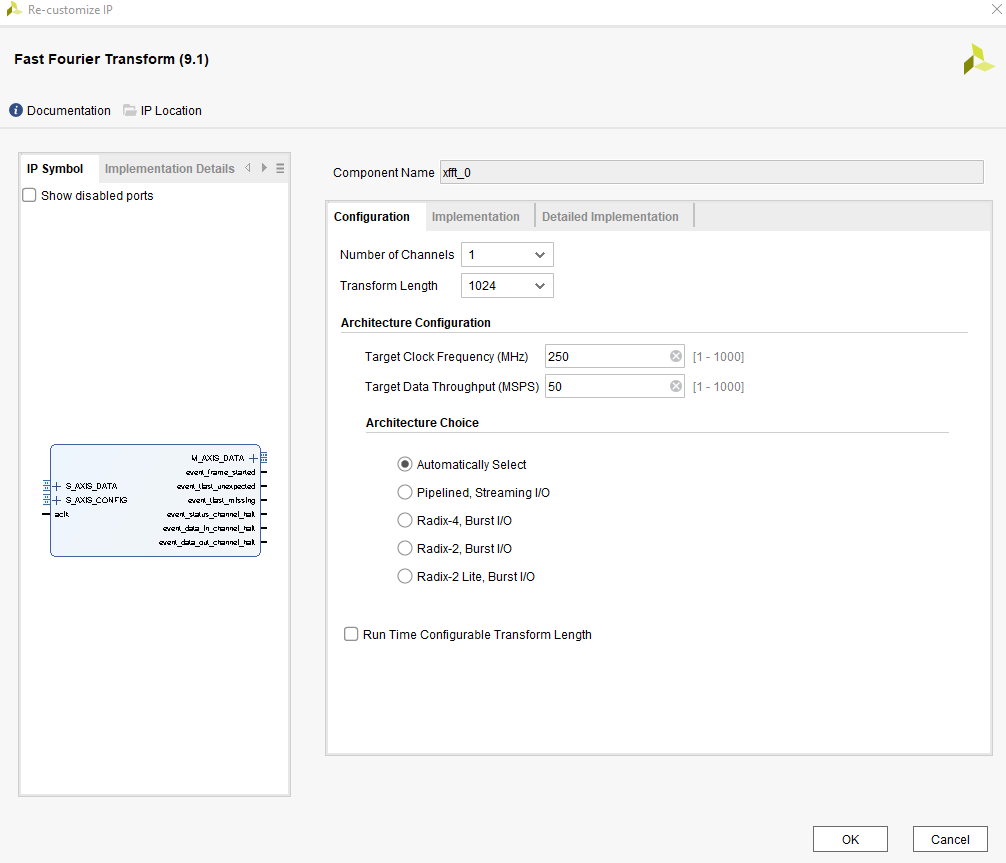
\includegraphics[width=0.5\textwidth]{image/fft_config.png}
	\caption{Временная диаграмма работы интерфейса AXI4-Stream}
	\label{fft_config}
\end{figure}
	
\begin{figure}[h]
	\centering
	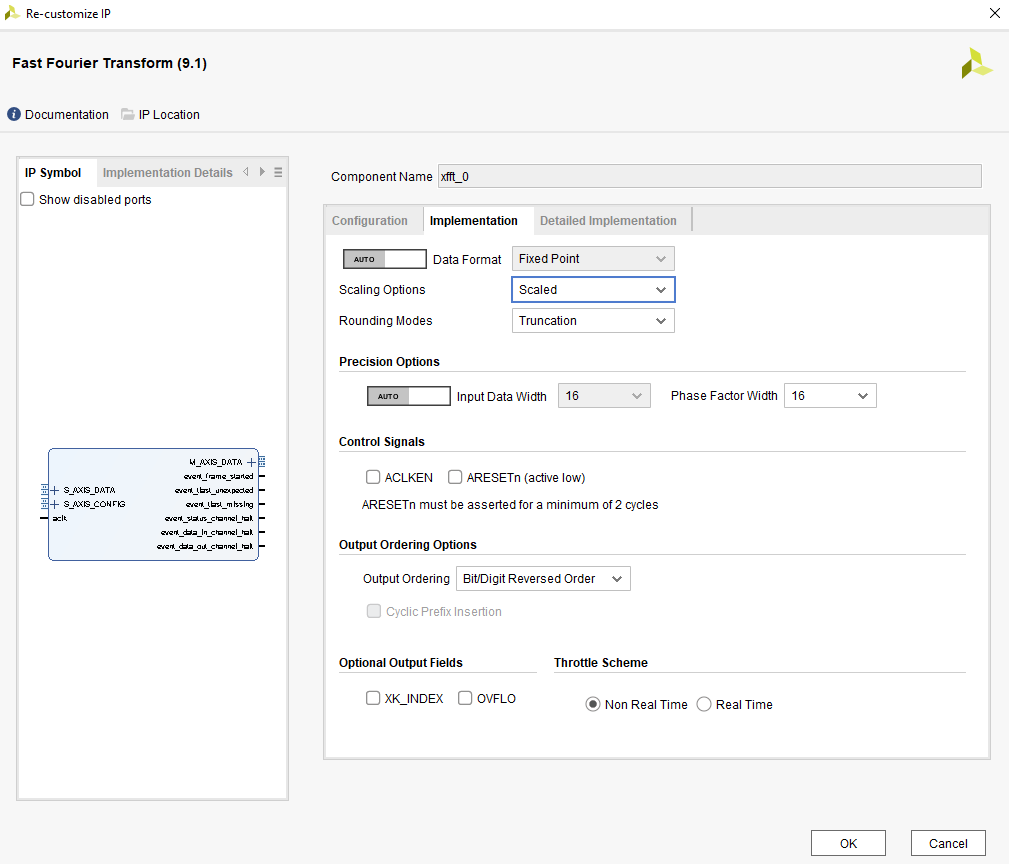
\includegraphics[width=0.5\textwidth]{image/fft_implemetation.png}
	\caption{Временная диаграмма работы интерфейса AXI4-Stream}
	\label{fft_implemetation}
\end{figure}
	
\section{Практическая часть}

Вкладка Configuration содержит:
\begin{enumerate}
	\item Число одновременно обрабатываемых каналов: выберите количество каналов от 1 до 12. Многоканальный режим доступен только для архитектур Burst I/O.
	\item Размер вектора преобразуемых данных: от 8 до 65536 отсчётов.
	\item Выбор архитектуры ядра.
	\item Параметры длины преобразования: выберите длину преобразования, которая будет настраиваться во время выполнения или нет. Ядро использует меньше логических ресурсов и имеет более высокую максимальную тактовую частоту, когда длина преобразования не настраивается во время выполнения.
\end{enumerate}

Вкладка «Реализация»
\begin{enumerate}
\item Формат данных: выберите, будут ли выборки входных и выходных данных в фиксированной точке или в формате с плавающей запятой одинарной точности IEEE-754 (32 бита). Плавающая точка
формат недоступен, когда ядро находится в многоканальной конфигурации.
\item Параметры точности: входные данные и фазовые коэффициенты можно настроить независимо друг от друга.разрядность от 8 до 34 бит включительно. Когда формат данных - с плавающей запятой, входширина данных фиксируется на уровне 32 бит, а ширина фазового коэффициента может быть установлена на 24 или 25 битов зависимости от требуемой шумовой производительности и доступных ресурсов.


\item Параметры масштабирования. Доступны три параметра для всех архитектур:
° Немасштабированный
- Все целочисленные разряды передаются на выход. Это может использовать больше FPGA Ресурсы.
° В масштабе
- Определяемый пользователем график масштабирования определяет, как данные масштабируются между БПФ и
этапы.
° Блок с плавающей запятой
- Ядро определяет, насколько масштабирование необходимо для наилучшего использования
доступный динамический диапазон и сообщает масштабный коэффициент в виде блочной экспоненты.
\item Сигналы управления: Включение часов (aclken) и Синхронный сброс (aresetn)
дополнительные штифты. Synchronous Clear имеет приоритет над Clock Enable, если выбраны оба параметра. Если
опция не выбрана, некоторые логические ресурсы могут быть сохранены и более высокая тактовая частота
может быть достижимо.
\item Необязательные поля вывода: \verb|XK_INDEX| является необязательным полем в канале вывода данных.
OVFLO является необязательным полем как в канале вывода данных, так и в канале состояния.
\item Схемы дросселирования: выбор компромисса между производительностью и синхронизацией данных.
требования. Режим реального времени обычно дает меньший и более быстрый дизайн, но имеет строгие ограничения.
ограничения на то, когда данные должны быть предоставлены и использованы. Режим не в реальном времени не имеет
такие ограничения, но дизайн может быть больше и медленнее. См. Управление БПФ.
Ядро для более подробной информации.
\item Режимы округления: на выходе бабочки младшие биты в тракте данных должны быть
подстриженный. Эти биты могут быть усечены или округлены с использованием конвергентного округления, которое
беспристрастная схема округления. Когда дробная часть числа точно равна
до половины, сходящееся округление округляет в большую сторону, если число нечетное, и округляет в меньшую, если
число четное. Конвергентное округление можно использовать, чтобы избежать смещения постоянного тока, которое могло бы
в противном случае вводите путем усечения после стадий бабочки. Выбор этой опции
увеличивает использование слайсов и дает небольшое увеличение времени преобразования из-за дополнительных
задержка.
\item Порядок вывода: выбор выходных данных: битовый/цифровой обратный порядок или естественный.
Заказ. Архитектуры на основе Radix-2 (конвейерный потоковый ввод-вывод, пакетный ввод-вывод Radix-2 и
Radix-2 Lite Burst I/O) предлагает обратный порядок битов и архитектуру на основе Radix-4.
(Radix-4 Burst I/O) предлагает обратный порядок цифр. Для конвейерного потокового ввода-вывода
архитектуре выбор естественного порядка вывода приводит к увеличению объема памяти
используется ядром. Для архитектур Burst I/O выбор выходных данных в естественном порядке увеличивает
общее время преобразования, поскольку требуется отдельная фаза разгрузки.
\item Циклическая вставка префикса может быть выбрана, если выходной порядок соответствует естественному порядку. Циклический
Вставка префикса доступна для всех архитектур и обычно используется в OFDM.
системы беспроводной связи.
\end{enumerate}

Информационные вкладки:
\begin{enumerate}
	\item Детали реализации:
	\begin{enumerate}
		\item Реализация: В этом поле отображается выбранная в данный момент архитектура. Это полезно увидеть результат автоматического выбора архитектуры.
		\item  Размер преобразования: когда длина преобразования настраивается во время выполнения, ядро возможность перепрограммирования размера точек во время работы ядра; то есть ядро может поддерживают выбранный размер точки и любой меньший размер точки. В этом поле отображается
		поддерживаемые размеры точек на основе длины преобразования, параметров длины преобразования,
		и выбранные варианты реализации.

		\item Ширина выходных данных: ширина выходных данных равна ширине входных данных для
		арифметика и блочная арифметика с плавающей запятой. При немасштабированной арифметике вывод
		ширина данных равна (ширина входных данных + log2 (размер точки) + 1).
		\item Оценки ресурсов: в зависимости от выбранных параметров в этом поле отображается срез DSP.
		count и 18K блоков ОЗУ. Количество ресурсов является лишь оценкой. За точное использование ресурсов и информацию о паре слайс/LUT-FlipFlop, следует ознакомиться с отчетом об использовании после внедрения.
		\item Структура порта AXI4-Stream: в этом разделе показано, как поля БПФ каналы AXI.
	\end{enumerate}
\item Задержка: На этой вкладке отображается задержка ядра БПФ в тактовых циклах и микросекундах (мкс) для
поддерживается каждый размер точки. Задержка исходит от вышестоящего мастера, поставляющего
от первой выборки кадра до последней выборки выходных данных, выходящих из ядра, предполагая, что ядро FFT простаивало и ни восходящий мастер, ни Ведомый нисходящий поток вставил состояния ожидания. Это не минимальное количество циклов между начальными последовательными кадрами, поскольку в некоторых случаях кадры могут перекрываться задержка в микросекундах зависит от целевой тактовой частоты.
\end{enumerate}

\subsection{Моделирование подсистемы сжатия сигналов}

\begin{Verbatim}[tabsize=4]
`timescale 1 ns/1 ps

module ham_tb();

reg aclk_reg;
reg aresetn_reg;

wire           FFT_CONFIG_tready;
wire           IFFT_CONFIG_tready;
wire           FFT_SF_CONFIG_tready;
wire           S_AXIS_IM_tready;
wire           S_AXIS_RE_tready;

wire           SF_IM_tready;
wire           SF_RE_tready;

reg [15:0]     FFT_CONFIG_tdata_reg;
reg            FFT_CONFIG_tvalid_reg;

reg [23:0]     IFFT_CONFIG_tdata_reg;
reg            IFFT_CONFIG_tvalid_reg;

reg [15:0]     S_AXIS_IM_tdata_reg;
reg            S_AXIS_IM_tlast_reg;
reg            S_AXIS_IM_tvalid_reg;

reg [15:0]     S_AXIS_RE_tdata_reg;
reg            S_AXIS_RE_tlast_reg;
reg            S_AXIS_RE_tvalid_reg;

reg [63:0]     S_AXIS_SF_tdata_reg;
reg            S_AXIS_SF_tvalid_reg;

reg [15:0]     SF_RE_tdata_reg;
reg [15:0]     SF_IM_tdata_reg;

reg            SF_RE_tvalid_reg;
reg            SF_IM_tvalid_reg;

reg [15:0]     FFT_SF_CONFIG_tdata_reg;
reg            FFT_SF_CONFIG_tvalid_reg;

design_1_wrapper
design_1_wrapper_inst
(
   .FFT_SF_CONFIG_tdata(FFT_SF_CONFIG_tdata_reg),
   .FFT_SF_CONFIG_tready(FFT_SF_CONFIG_tready),
   .FFT_SF_CONFIG_tvalid(FFT_SF_CONFIG_tvalid_reg),

   // Настройка БПФ ядра  
   .FFT_CONFIG_tdata(FFT_CONFIG_tdata_reg),
   .FFT_CONFIG_tready(FFT_CONFIG_tready),
   .FFT_CONFIG_tvalid(FFT_CONFIG_tvalid_reg),

   // Настройка ОБПФ ядра
   .IFFT_CONFIG_tdata(IFFT_CONFIG_tdata_reg),
   .IFFT_CONFIG_tready(IFFT_CONFIG_tready),
   .IFFT_CONFIG_tvalid(IFFT_CONFIG_tvalid_reg),

   .M_AXIS_DATA_tdata(),
   .M_AXIS_DATA_tlast(),
   .M_AXIS_DATA_tready(1'b0),
   .M_AXIS_DATA_tvalid(),
   
   .S_AXIS_IM_tdata(S_AXIS_IM_tdata_reg),
   .S_AXIS_IM_tlast(S_AXIS_IM_tlast_reg),
   .S_AXIS_IM_tvalid(S_AXIS_RE_tvalid_reg),
   .S_AXIS_IM_tready(S_AXIS_IM_tready),
   
   .S_AXIS_RE_tdata(S_AXIS_RE_tdata_reg),
   .S_AXIS_RE_tlast(S_AXIS_RE_tlast_reg),
   .S_AXIS_RE_tvalid(S_AXIS_RE_tvalid_reg),
   .S_AXIS_RE_tready(S_AXIS_RE_tready),
    
   .SF_IM_tdata(SF_IM_tdata_reg),
   .SF_IM_tready(SF_IM_tready),
   .SF_IM_tvalid(SF_IM_tvalid_reg),
   
   .SF_RE_tdata(SF_RE_tdata_reg),
   .SF_RE_tready(SF_RE_tready),
   .SF_RE_tvalid(SF_RE_tvalid_reg),

   .aclk(aclk_reg),
   .aresetn(aresetn_reg)
);


initial begin
   aclk_reg = 0;
   forever begin
      #5;
      aclk_reg = !aclk_reg;
   end
end

integer fd_recv_re;
integer fd_recv_im;  

integer fd_recv_int16_re;
integer fd_recv_int16_im;  

reg [15:0] lfm_reg;

reg [15:0] lfm_re_shift_reg [1023:0];
reg [15:0] lfm_im_shift_reg [1023:0];

reg [15:0] lfm_re_int16_reg [1023:0];
reg [15:0] lfm_im_int16_reg [1023:0];

initial begin
   $display("Read LFM from files ...");

   fd_recv_re = $fopen("lfm_int16_shift_re.dat","rb");
   fd_recv_im = $fopen("lfm_int16_shift_im.dat","rb");
   $fread(lfm_re_shift_reg, fd_recv_re);
   $fread(lfm_im_shift_reg, fd_recv_im);

   fd_recv_int16_re = $fopen("lfm_re_int16.dat","rb");
   fd_recv_int16_im = $fopen("lfm_im_int16.dat","rb");
   $fread(lfm_re_int16_reg, fd_recv_int16_re);
   $fread(lfm_im_int16_reg, fd_recv_int16_im);

   $display("Begin verification of correl function windows ...");
   aresetn_reg = 0;
   S_AXIS_SF_tdata_reg = 64'b0;
   S_AXIS_SF_tvalid_reg = 1'b0;

   S_AXIS_IM_tdata_reg = 16'b0;
   S_AXIS_IM_tlast_reg = 1'b0;
   S_AXIS_IM_tvalid_reg = 1'b0;

   S_AXIS_RE_tdata_reg = 16'b0;
   S_AXIS_RE_tlast_reg = 1'b0;
   S_AXIS_RE_tvalid_reg = 1'b0;

   FFT_CONFIG_tdata_reg = 16'b0;
   FFT_CONFIG_tvalid_reg = 1'b0;
   IFFT_CONFIG_tdata_reg = 24'b0;
   IFFT_CONFIG_tvalid_reg = 1'b0;
   FFT_SF_CONFIG_tdata_reg = 16'b0;
   FFT_SF_CONFIG_tvalid_reg = 1'b0;

   SF_IM_tvalid_reg = 0;
   SF_RE_tvalid_reg = 0;
   SF_RE_tdata_reg = 16'b0;
   SF_IM_tdata_reg = 16'b0;
   #100;
   aresetn_reg = 1;
   #250;
   
   // Задаём настройки для БПФ
   $display("FFT_CONFIG_tready event");
   wait(FFT_SF_CONFIG_tready);
   FFT_SF_CONFIG_tdata_reg = {15'b0, 1'b1};
   @(posedge aclk_reg);
   FFT_SF_CONFIG_tvalid_reg = 1'b1;
   @(posedge aclk_reg);
   FFT_SF_CONFIG_tvalid_reg = 1'b0;

   // Задаём настройки для БПФ
   $display("FFT_CONFIG_tready event");
   wait(FFT_CONFIG_tready);
   FFT_CONFIG_tdata_reg = {15'b0, 1'b1};
   @(posedge aclk_reg);
   FFT_CONFIG_tvalid_reg = 1'b1;
   @(posedge aclk_reg);
   FFT_CONFIG_tvalid_reg = 1'b0;

   // Задаём настройки для ОБПФ
   $display("IFFT_CONFIG_tdata_reg event");
   wait(IFFT_CONFIG_tready);
   IFFT_CONFIG_tdata_reg = {18'b0 , 1'b0, 5'b01010};
   @(posedge aclk_reg);
   IFFT_CONFIG_tvalid_reg = 1'b1;
   @(posedge aclk_reg);
   IFFT_CONFIG_tvalid_reg = 1'b0;

   // Задаём опорную функцию для сжатия
   // Задаём принятый сигнал для сжатия

   wait(SF_RE_tready);
   wait(SF_IM_tready);
   wait(S_AXIS_RE_tready);
   @(posedge aclk_reg);
   #9.9;
   SF_RE_tdata_reg = lfm_re_int16_reg[0];
   SF_IM_tdata_reg = lfm_im_int16_reg[0];
   S_AXIS_RE_tdata_reg = lfm_re_shift_reg[0];
   S_AXIS_IM_tdata_reg = lfm_im_shift_reg[0]; 
   SF_IM_tvalid_reg = 1;
   SF_RE_tvalid_reg = 1;
   S_AXIS_RE_tvalid_reg = 1;
   @(posedge aclk_reg);
   for (integer i = 1; i < 1024; i = i + 1) begin
      @(posedge aclk_reg);
      SF_RE_tdata_reg = lfm_re_int16_reg[i];
      SF_IM_tdata_reg = lfm_im_int16_reg[i];
      S_AXIS_RE_tdata_reg = lfm_re_shift_reg[i];
      S_AXIS_IM_tdata_reg = lfm_im_shift_reg[i]; 
   end
   #9.9;   
   SF_RE_tvalid_reg = 0;
   SF_IM_tvalid_reg = 0;
   S_AXIS_RE_tvalid_reg = 0;

   $display("TEST PASSED");
end

endmodule
\end{Verbatim}

\begin{figure}[h]
	\centering
	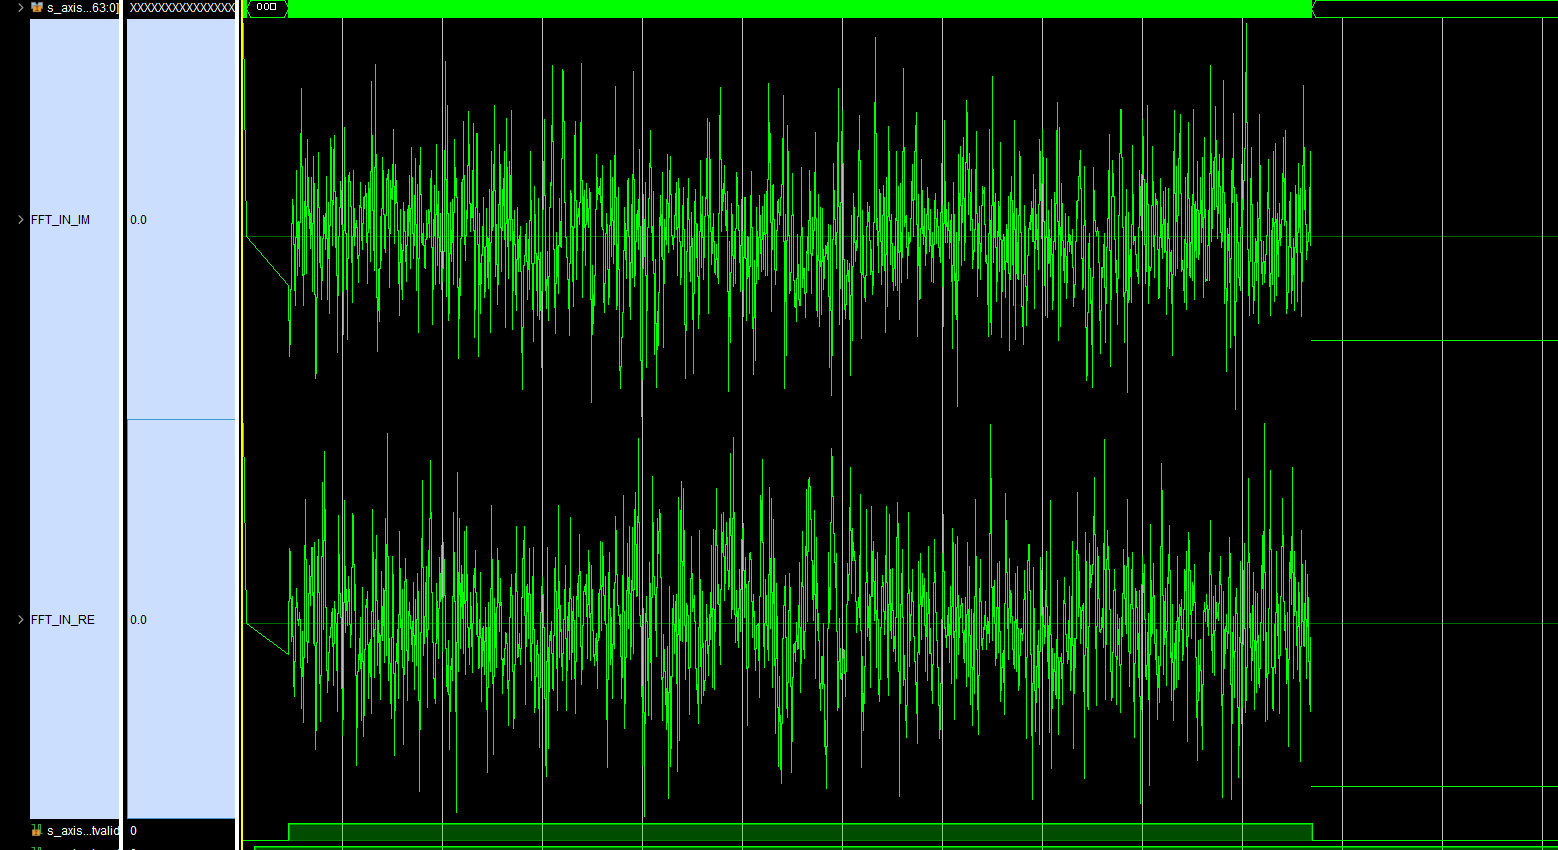
\includegraphics[width=0.5\textwidth]{image/lfm_with_noise.png}
	\caption{Временная диаграмма работы интерфейса AXI4-Stream}
	\label{fft_result}
\end{figure}
	
\begin{figure}[h]
	\centering
	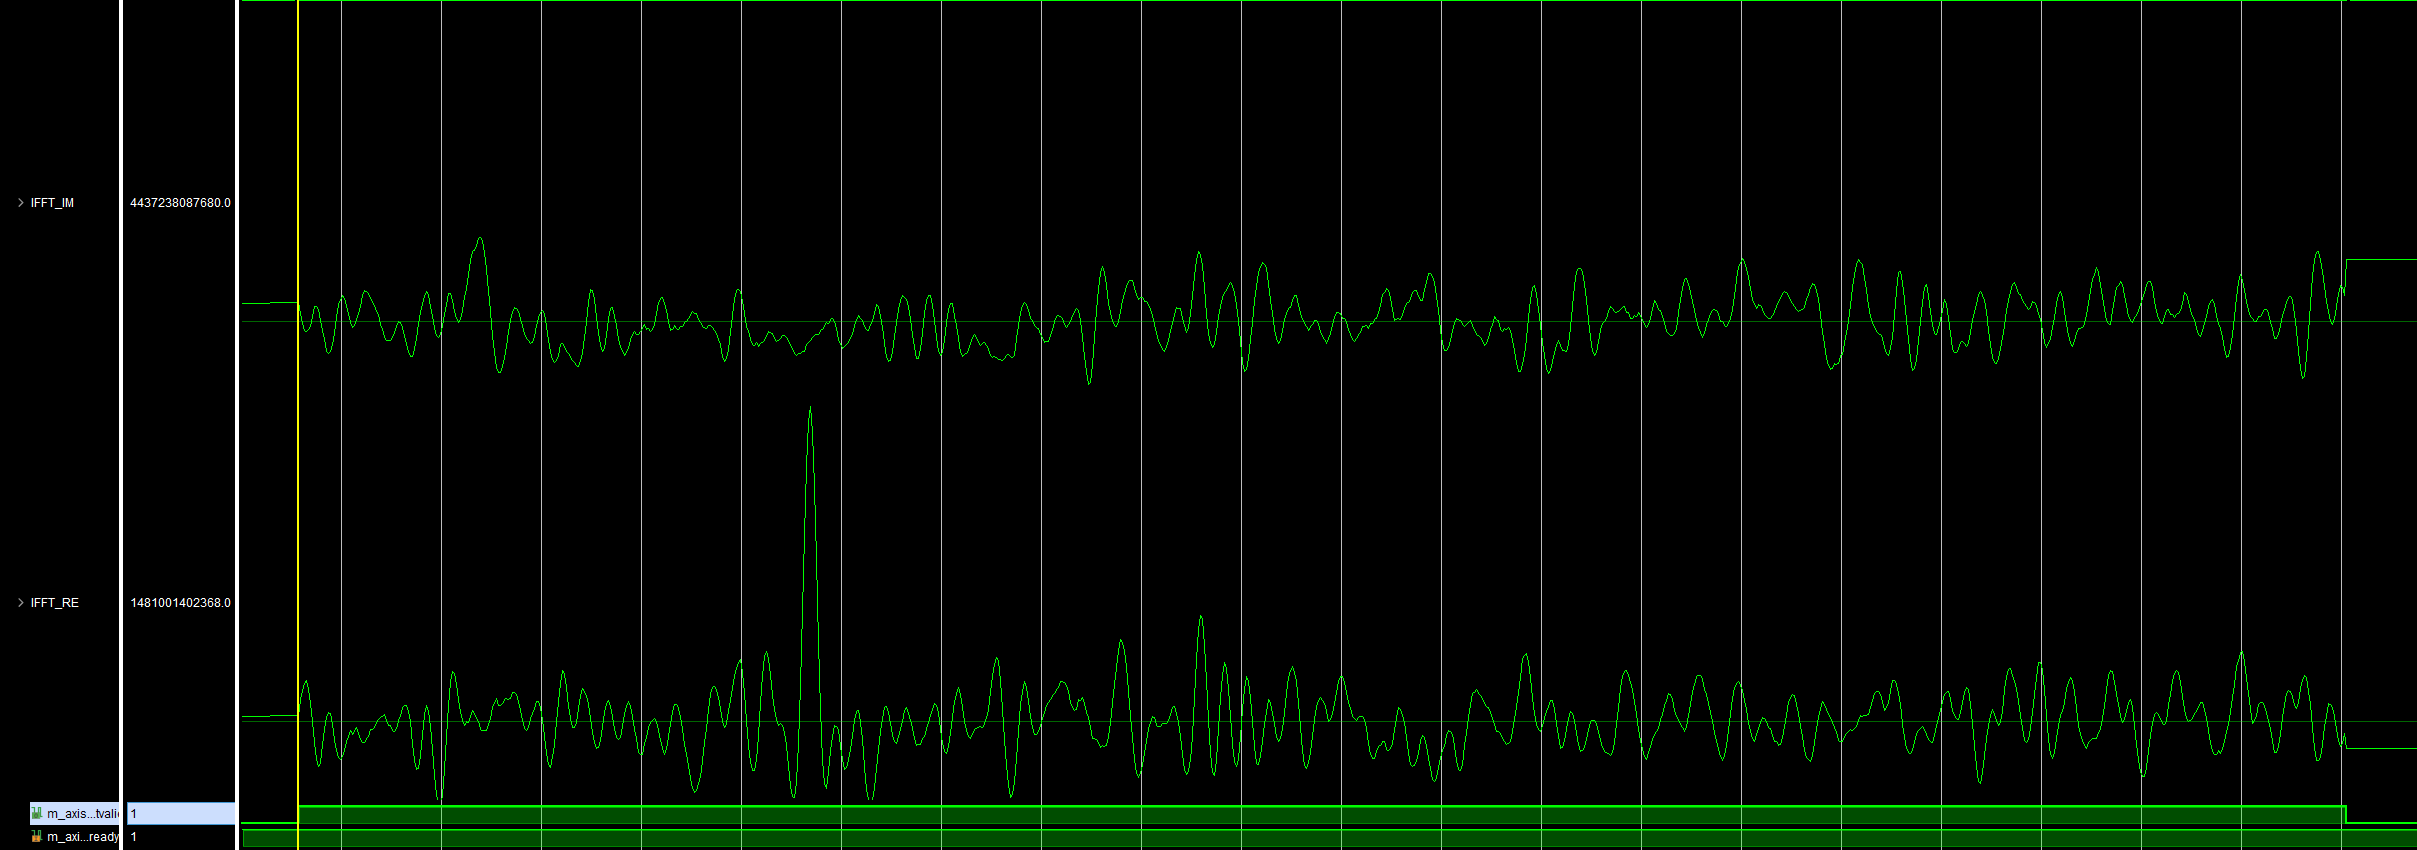
\includegraphics[width=0.5\textwidth]{image/correl_with_noise.png}
	\caption{Временная диаграмма работы интерфейса AXI4-Stream}
	\label{fft_detailed_implem}
\end{figure}

